\chapter{The GOTO Telescope Control System}
\label{chap:gtecs}
\chaptoc{}

% ########################################

\newpage
\section{Introduction}
\label{sec:gtecs_intro}
\begin{colsection}

% ~~~~~~~~~~~~~~~~~~~~

\begin{colsection}

\rtxt{TODO}

In this chapter I outline my work creating a control system for the GOTO telescope. \aref{chap:gtecs}, \aref{chap:autonomous} and \aref{chap:scheduling} are expanded from my SPIE conference paper \citealt{Dyer}. The GOTO Telescope Control System is based on the pt5m control system (\citealt{pt5m}), written primarily by Tim Butterly at Durham and Stu Littlefair and Vik Dhillon at Sheffield. This provided the foundation that the GOTO system builds upon, but has been heavily modified and rewritten to meet the requirements of the GOTO project. All work described in this chapter is my own, incorporating advice and feedback from members of the GOTO collaboration.

\end{colsection}

% ~~~~~~~~~~~~~~~~~~~~

\subsection{Requirements of the control system}
\label{sec:control_requirements}
\begin{colsection}

My first task as part of the GOTO collaboration, in the summer of 2015 before I started my PhD in Sheffield, was to decide on what control system software to use for the telescope. There were several requirements to consider.

First, the chosen system had to allow for remote and, most importantly, robotic operation of GOTO.\@ There are many telescope control software packages available, but the majority are designed for a human observer to operate. GOTO however was to be a fully autonomous telescope, which meant operating nightly with no human intervention. This meant the control system had to contain routines for observing targets and standard tasks like taking calibration frames. On top of that it was desirable for the system to be able to monitor itself to detect and fix any errors as much as possible without the need for human intervention. Finally it had to be able to monitor and react to external conditions, for example closing the dome if rain was detected.

Second, the system had to include an observation scheduler, which could decide what the telescope should observe during the night. A basic scheduler might be run in the evening to create a night plan, as observers typically do when operating a telescope. However that function alone would not meet the expected operations required from GOTO:\@ normally carrying out an all-sky survey but with a robust interrupt protocol for gravitational wave follow-up. The system therefore had to be able to recalculate what to observe on-the-fly, and be able to react immediately to transient \gls{too} events.

Furthermore, although the project was still at an early stage the idea of linking together multiple telescopes into a global network was also considered, and the chosen control system would ideally be expandable to facilitate this in the future.

There were also several physical considerations when it came to choosing between software systems. The telescope hardware had already been decided on: an Astrohaven clamshell dome\footnote{Astro Haven Enterprises, CA, USA;\@ (\url{www.astrohaven.com})}, a custom mount with a \gls{sitech} servo controller\footnote{Sidereal Technology, OR, USA;\@ (\url{www.siderealtechnology.com})} and multiple unit telescopes all equipped with \gls{fli} cameras, focusers and filter wheels\footnote{Fingerlake Instruments, NY, USA;\@ (\url{www.flicamera.com})}. Any control system would need to communicate with all of this hardware, so any software package with existing drivers would be desirable. \rtxt{in intro}

Two particular hardware-related challenges faced the control system project. The first was that the SiTech controller software, \software{SiTechEXE}, only ran on Microsoft Windows. The software did have an accessible \gls{api} through the \software{ASCOM} standard\footnote{\url{www.ascom-standards.org}}, but that still required some form of the mount control system to be running on Windows. As most professional scientific software in astronomy runs on Linux systems, this lead to two options: either have just a small interface running on the Windows machine and the rest of the system on Linux, or have the entire system run on Windows.

The second hardware-related challenge was to deal with the multiple-unit telescope design of \gls{goto}. A full array of eight unit telescopes (UTs) would require eight cameras, focusers and filter wheels. These would all need to be run in parallel, most importantly there needed to be no delay between the exposures starting and finishing on each camera. The physical construction of the telescope also came into play. The \gls{fli} units all require a USB connection to the control computer. A single computer situated in the dome would therefore require 24 extra-long USB cables to run up the mount. The suggested solution was to have small computers attached to the mount boom arms to act as intermediate interfaces to the \gls{ut} hardware \rtxt{shown in figure in intro}. The control system therefore needed to be able to run in a distributed manner across multiple computers, potentially even running different operating systems.

There were also practical details to consider when choosing the control software. \gls{goto} was designed as a relatively inexpensive project that could be built quickly and copied across multiple sites, therefore any costly software licenses should ideally be avoided. Experience and support requirements should also be considered, and reusing a software system that members of the collaboration had experience with would provide benefits compared to a completely new system.

\end{colsection}

% ~~~~~~~~~~~~~~~~~~~~

\subsection{Different control system options}
\label{sec:control_options}
\begin{colsection}

Four possible options for the GOTO control system were considered: the existing software packages \software{ACP Expert}, \software{Talon} and \software{RTS2}, or a custom system based on the code written for the \gls{pt5m}. At the July 2015 GOTO meeting at Warwick University I gave a talk outlining the control system requirements and presenting the four options, and the decision taken was to adapt the \gls{pt5m} system for use by GOTO.\@ The three rejected systems are described below, while the \gls{pt5m} system is described in more detail in \aref{sec:pt5m}.

\subsubsection{\software{ACP Expert}}
\software{ACP Expert}\footnote{\url{http://acp.dc3.com}} is a commercial observatory control software system by DC3-Dreams. It is used by some advanced amateur astronomers and a few scientific and university telescopes, such as the Open University's \gls{pirate} \citep{PIRATE}. As a complete Windows software package with a web interface it is marketed as being straightforward to use, in either remote or fully robotic modes. It uses the \software{ASCOM} standard library and DC3-Dreams also provide professional support and updates. This however came at a cost: \$2495 for the base software, plus an additional \$599 for Maxim DL camera control and \$650 per year for continued support. At the time, \gls{goto} was anticipated to be deployed in a matter of months, so the quick and simple pre-existing commercial solution was tempting. However it was unclear if the \software{ACP} software would be able to cope with \gls{goto}'s unusual design, and its closed-source model would restrict our ability to make modifications.

\subsubsection{\software{Talon}}

The \software{Talon} observatory control system\footnote{\url{https://observatory.sourceforge.io}} is a Linux-based, open-source system created by \gls{omi}. It was included as an option primarily as at the time it was the control system of choice for the other observatories operated by Warwick University, such as SuperWASP \citep{SuperWASP}. \gls{omi} had built the SuperWASP mount and developed \software{Talon} alongside it, before later making it open source. However development of \software{Talon} has been almost non-existent over the past decade, and when building the \gls{ngts} a large amount of custom software was needed to allow \software{Talon} to work with its multiple telescopes \citep{ngts}. Warwick were already looking at replacing \software{Talon} for their \gls{w1m} and when upgrading SuperWASP.\@ Therefore adopting it for \gls{goto} would be unlikely and even counter-productive, as whatever was chosen for \gls{goto} was expected to (and ultimately did) influence and benefit the concurrent development of a new control system for \gls{w1m}.

\subsubsection{\software{RTS2}}

The \gls{rts2}\footnote{\url{https://rts2.org}} \citep{RTS2, RTS2b} is another free and open-source Linux software package. Unlike \software{Talon}, \software{RTS2} is under active development and is used by telescopes and observatories around the world \citep{BORAT, BOOTES-3, antarctic, ARTN}. There is a small but active user community and drivers for the hardware \gls{goto} would use had already been developed. The first version of RTS was written in \proglang{Python}, while the second version was rewritten in \proglang{C++} but with a \proglang{Python} interface available. \gls{rts2} was an attractive choice, however like the others it was unclear if it could be easily modified to meet the requirements for \gls{goto}'s multiple telescopes and Windows-controlled mount and no one in the collaboration had prior experience of using or implementing it.

\end{colsection}

% ~~~~~~~~~~~~~~~~~~~~

\subsection{The \textit{pt5m} control system}
\label{sec:pt5m}
\begin{colsection}

Built and operated by Sheffield and Durham Universities, \gls{pt5m} is a \SI{0.5}{\metre} telescope located on the roof of the \SI{4.2}{\metre} \gls{wht} on La Palma \citep{pt5m}. The telescope was originally developed as a \gls{slodar} system for atmospheric turbulence profiling in support of the CANARY laser guide star project on the \gls{wht} \citep{SLODAR_LaPalma, CANARY}. There are several \gls{slodar} telescopes around the world operated by Durham, including one in Korea that had just been commissioned at the time I joined the GOTO project \citep{SLODAR_Korea}. In order to make the most of the telescope when not being used for \gls{slodar} observations a science camera was added to \gls{pt5m} by Sheffield, and in-house control software was written to enable robotic observations. It has successfully been used for automatic observations of transient events since 2012, as well as being used for undergraduate teaching at Sheffield and Durham. All of the \gls{slodar} telescopes used a custom control system developed at Durham, and a similar system was used by the teaching telescopes of the Durham Department of Physics that I worked with during my undergraduate program. The \gls{pt5m} control system had been modified by the team at Durham and Sheffield for robotic operation, which matched well with what we needed for \gls{goto}. For this reason, on top of the existing experience of the software, it was chosen to be the base for the GOTO control system.

The \gls{pt5m} control system is written in \proglang{Python} and was built around multiple independent background programs called \emph{daemons}. Each daemon controls one category of hardware, for example the dome, mount or CCD controller. A script called the \emph{pilot} sends commands to the daemons when the system is operating in robotic mode, and the decision of what to observe is taken by the \emph{scheduler} which picks targets out of a database and returns the highest priority to the pilot. Finally a separate script called the \emph{conditions monitor} checks the local weather conditions and tells the pilot to close the dome in bad weather. An overview of the pt5m control system architecture is shown in \aref{fig:pt5m_software}.

The basic framework of the pt5m control system was adopted for \gls{goto}, but with several changes. The major difference between \gls{pt5m} and \gls{goto} are the multiple unit telescopes, but the same software control system could be adapted through the creation of interface daemons which allow communication to the unit telescopes over the internal dome network. In fact the independent, distributed nature of the daemon system made it very easy to expand to have daemons running on physically separate machines but still communicating over the same local network, including on both Linux and Windows computers.

\begin{figure}[p]
    \begin{center}
        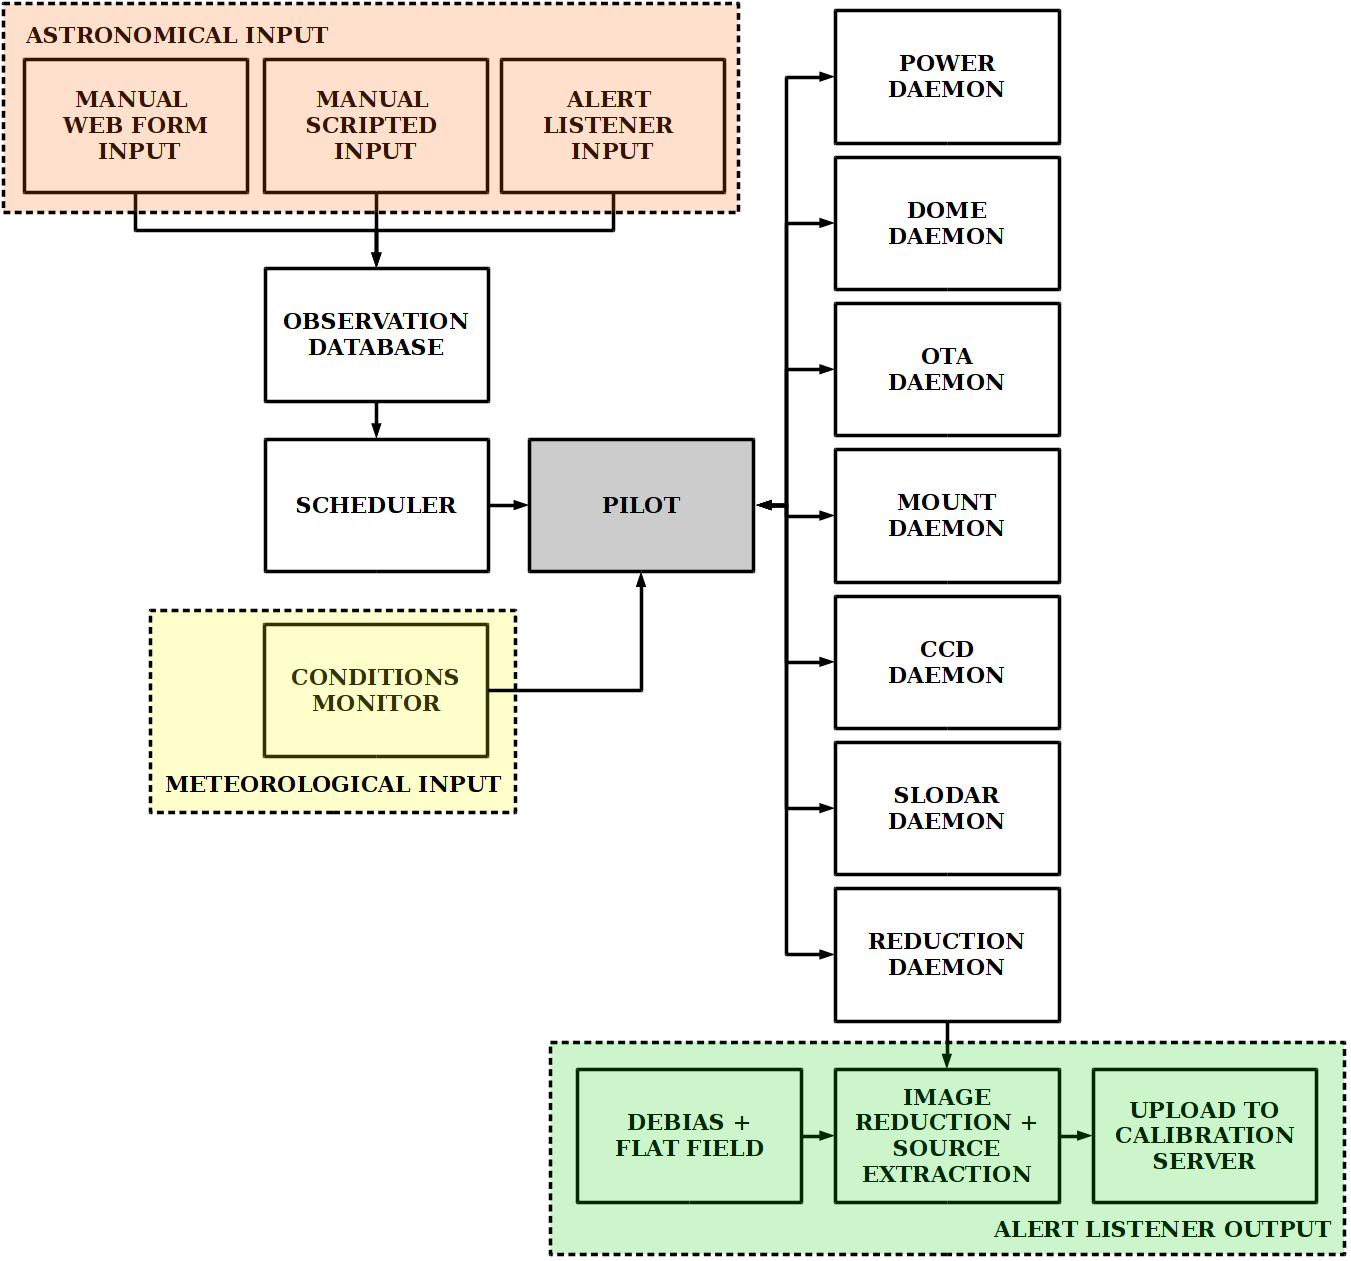
\includegraphics[width=\linewidth]{images/pt5m_software.png}
    \end{center}
    \caption[The pt5m control system architecture]{
        The \gls{pt5m} control system architecture, taken from \citet{pt5m}. The hardware daemons are shown on the right; they communicate with the pilot which receives information from the observation scheduler and the conditions monitor. This basic framework was adapted for the GOTO control system, c.f. \aref{fig:flow}.
    }\label{fig:pt5m_software}
\end{figure}

\end{colsection}

% ~~~~~~~~~~~~~~~~~~~~

\end{colsection}

% ########################################

\newpage
\section{Overview of G-TeCS}
\label{sec:gtecs}
\begin{colsection}

% ~~~~~~~~~~~~~~~~~~~~

\begin{colsection}

\rtxt{TODO}

The \gls{gtecs} is the name given to the collection of programs that have been developed to fulfil the requirements of the GOTO project given in \aref{sec:control_requirements}. The \gls{pt5m} control system as described in the previous section formed the basis for \gls{gtecs}. Its structure of multiple independent daemons was developed into the core system architecture of G-TeCS, shown in \aref{fig:flow}. This section gives an overview of the system and its implementation, and the following sections discuss in detail the two core branches of G-TeCS:\@ the base hardware control programs (\aref{sec:hardware_control}) and the autonomous systems built on top of them (\aref{chap:autonomous}).

\begin{figure}[p]
    \begin{center}
        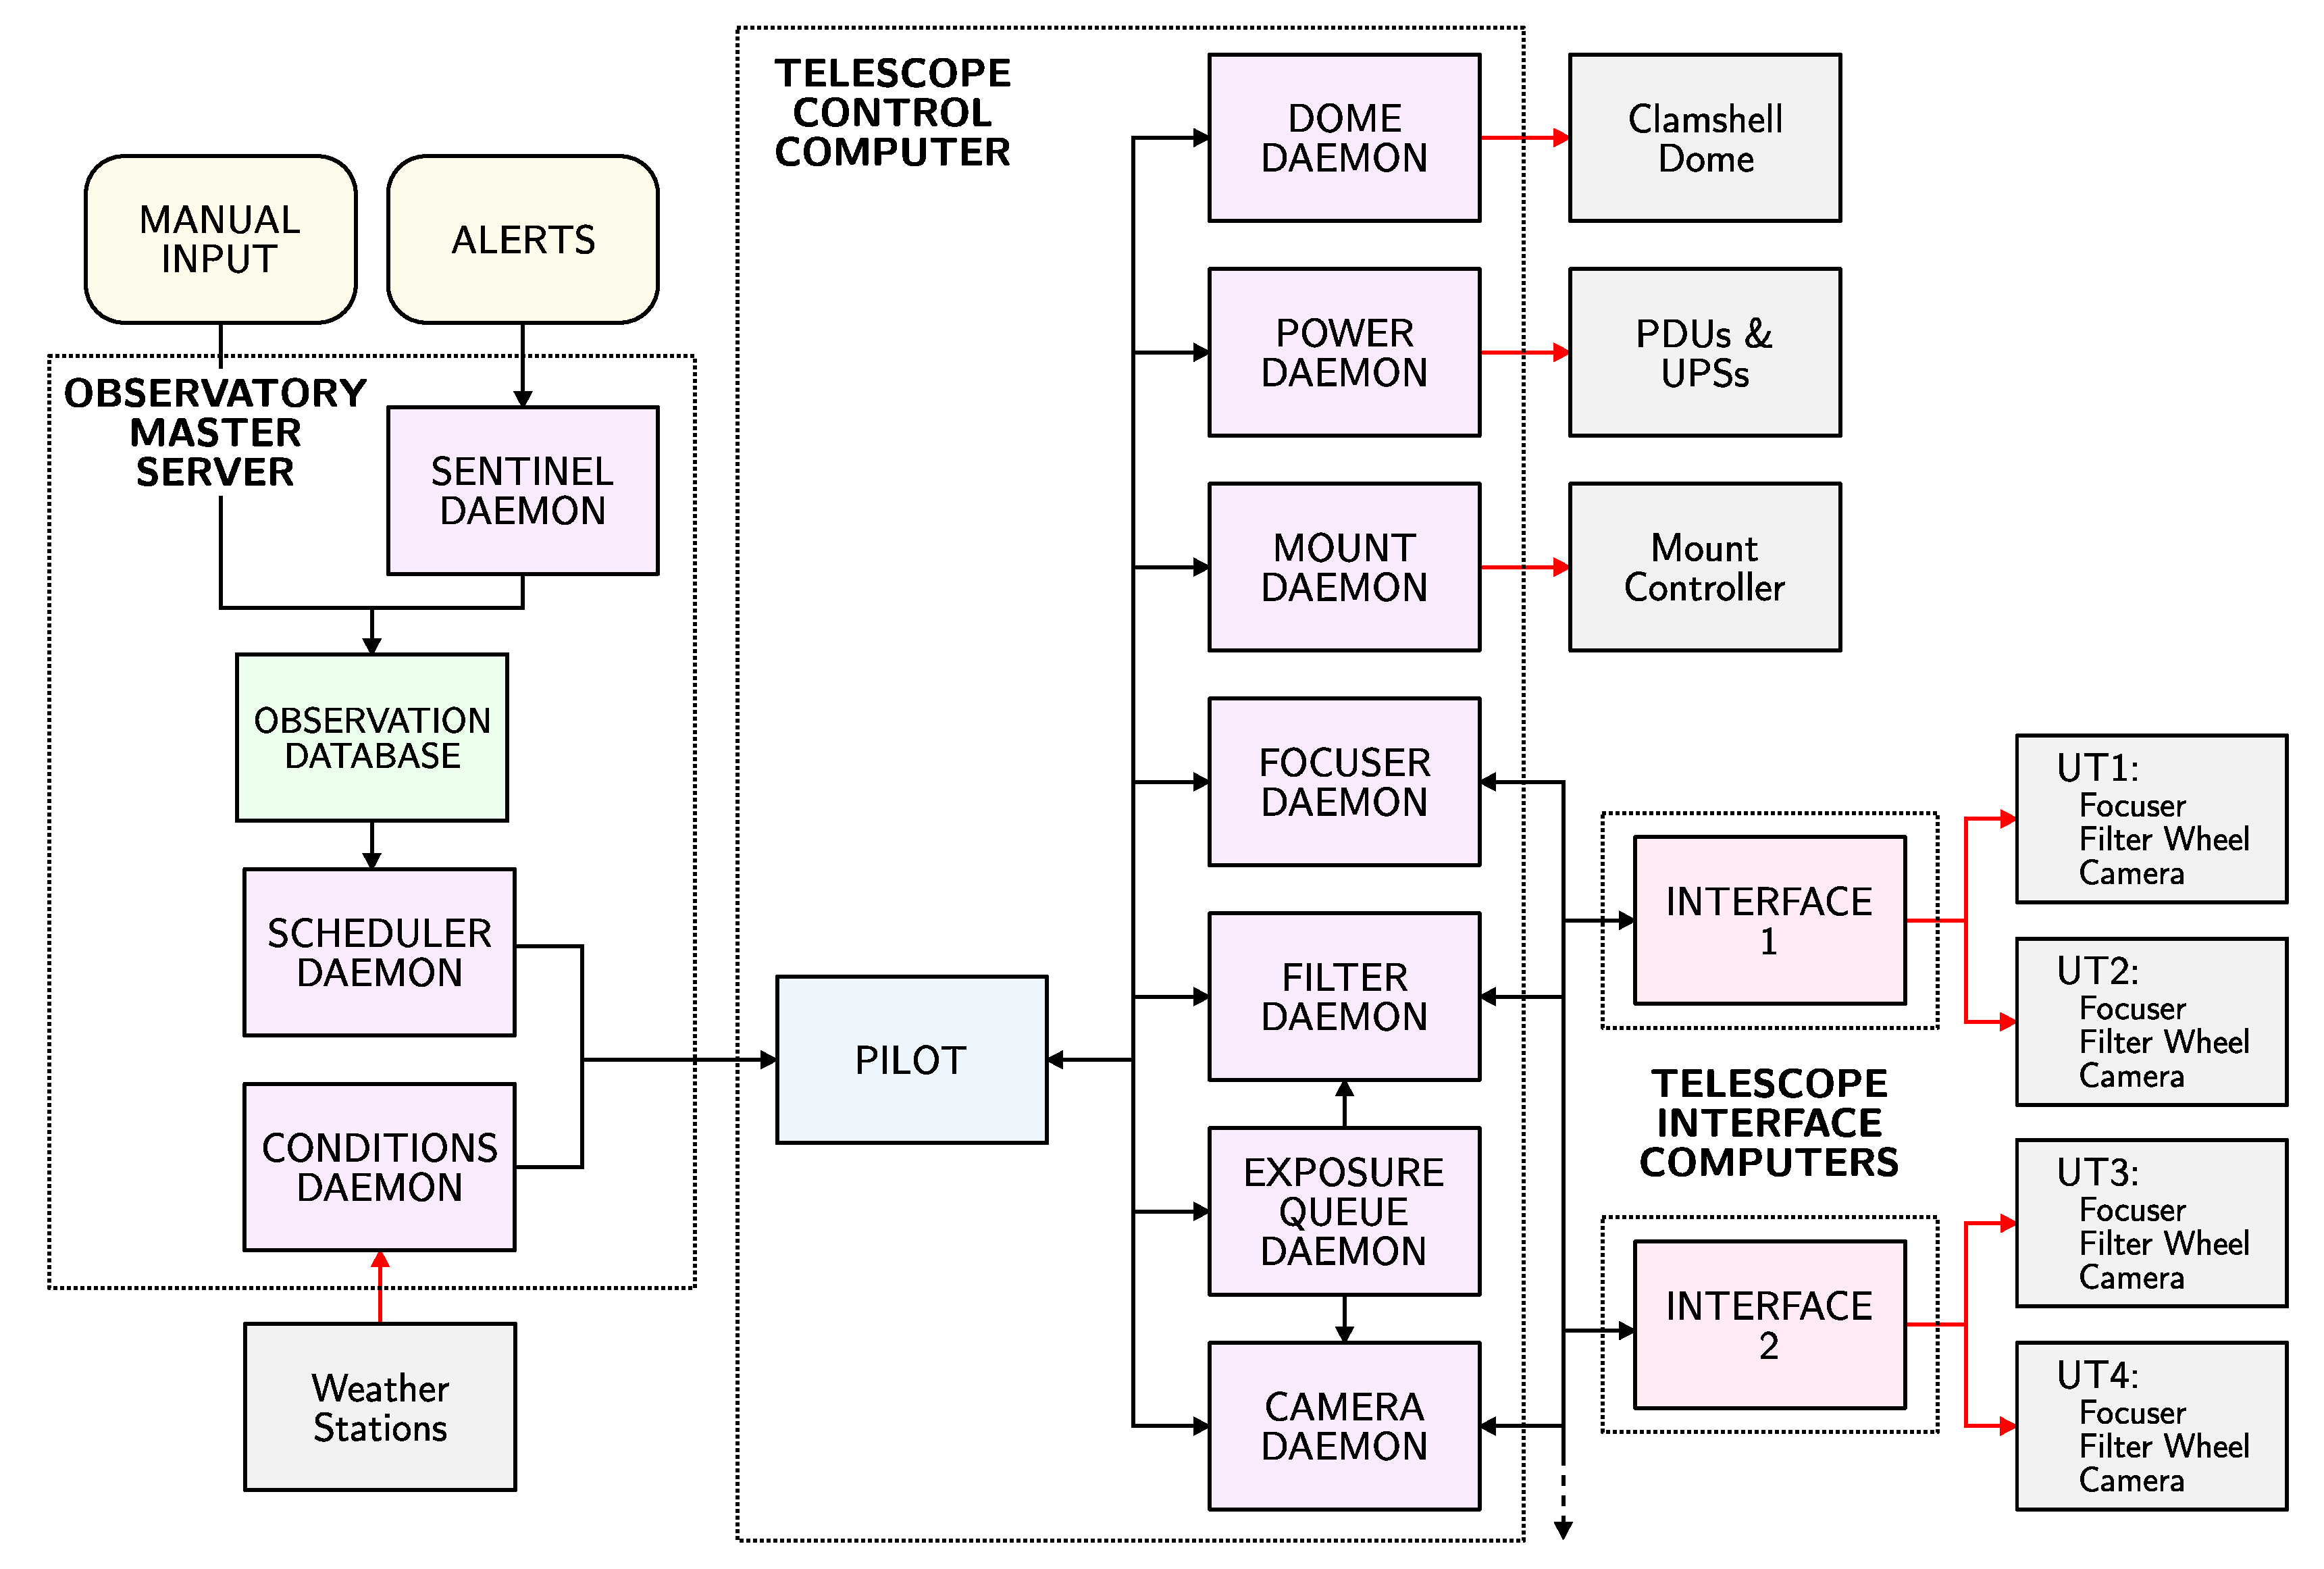
\includegraphics[width=\linewidth]{images/flow.pdf}
    \end{center}
    \caption[The G-TeCS system architecture]{
        The \gls{gtecs} system architecture as deployed on La Palma. The observation database as well as the sentinel, scheduler and conditions daemons shown to the left run on a central observatory-wide server located in the SuperWASP building next to the GOTO domes, while the pilot and hardware daemons are located on the telescope control computer within the dome. Control for the unit telescope hardware (focuser, filter wheel and camera) is sent via an interface daemon for each pair of UTs, running on computers attached to the mount. Only the system for the prototype instrument (one mount with four unit telescopes) is shown.
    }\label{fig:flow}
\end{figure}

\end{colsection}

% ~~~~~~~~~~~~~~~~~~~~

\subsection{Implementation}
\label{sec:implementation}
\begin{colsection}

The core \gls{gtecs} code is written as a \proglang{Python} package, \pkg{gtecs}. This includes all of the daemons, scripts, associated modules and functions. One core component, the code and functions to interact with the observation database (see \aref{sec:obsdb}), has been split off into a separate \proglang{Python} package ObsDB (\pkg{obsdb}); this was to allow other users to interact with the database without the need to install the entire \pkg{gtecs} package. In addition, the code for alert processing within the sentinel (see \aref{sec:sentinel}) is in a separate module, GOTO-alert (\pkg{gotoalert}). This is because it originated as a separate coding project developed by Alex Obradovic at Monash, that I then took over and integrated with the \gls{gtecs} sentinel. GOTO-alert is described in more detail in \aref{sec:gotoalert}.

G-TeCS and the associated packages are written almost entirely in \proglang{Python}, specifically \proglang{Python3}. \proglang{Python} is a versatile programming language that is increasingly common in astronomy, helped by the popular open-source Astropy Project \citep{astropy}. \proglang{Python} version 3.0 was released in 2008 and is infamously not backwards-compatible with \proglang{Python2}. The code for \gls{pt5m} was written in \proglang{Python2}, and therefore initially so was G-TeCS.\@ Over the subsequent years the G-TeCS code was re-written to be compatible with both \proglang{Python2} and \proglang{Python3}, which was possible due to the inbuilt \code{\_\_future\_\_} module in \proglang{Python2} and the \code{six} package. Eventually, the addition of new features added to \proglang{Python3}, such as the \pkg{asyncio} package (used heavily by the pilot) in version 3.5, and the imminent end-of-life of \proglang{Python2} in 2020 led to the dropping of \proglang{Python2} support. This is in line with most other scientific \proglang{Python} packages including \pkg{astropy}, which is no longer developed for \proglang{Python2}. % chktex 21

The \pkg{gtecs} and associated packages have multiple dependencies. Some of the most critical external packages (not included in the \proglang{Python} standard library) are \pkg{numpy} for mathematical and scientific structures, \pkg{astropy} for astronomical functions, \pkg{Pyro4} for communicating between daemons (see \aref{sec:daemons} below) \pkg{sqlalchemy} for \proglang{SQL} database management (see \aref{sec:obsdb}), \pkg{astroplan} for scheduling (see \aref{sec:scheduler}), \pkg{voeventparse} for handling VOEvents (see \aref{sec:voevents}) and \pkg{gototile}, a custom package written for GOTO for skymap processing (described in \aref{sec:gototile}).

\end{colsection}

% ~~~~~~~~~~~~~~~~~~~~

\subsection{Daemons}
\label{sec:daemons}
\begin{colsection}

The core elements of the control system are the daemons. A \emph{daemon} is a type of computer program that runs as a background process, continually cycling and awaiting any input from the user. This is in contrast to a \emph{script} which is run once (either by the system or a user), carries out a series of tasks in the foreground and then exits once it is completed. Common examples of daemons on a Unix-based system are \software{sshd}, which listens for and creates \gls{ssh} connections, and \software{cron}, which runs commands at predefined times. Incidentally both are used by G-TeCS:\@ \gls{ssh} commands are used to execute commands on remote machines and \software{cron} is used to run scripts like the pilot at a set time of day.

Daemons are the ideal form of software for hardware control. Once started each daemon runs continually as a background process, with a main control loop that repeats on a regular timescale (for the G-TeCS hardware daemons this is usually every \SI{0.1}{\second}). There are two primary tasks that are carried out within the loop by every daemon: monitoring the status of the hardware, and listening for and carrying out input commands. The former is typically not carried out every time the loop runs, because attempting to request and process the hardware status every \SI{0.1}{\second} would overwhelm the daemon and delay the loop. Instead the status checks are typically carried out every \SI{2}{\second}, or sooner if requested. By continually requesting the status of the hardware the daemon will detect very quickly if there are any problems, and should they be unable to reach their hardware they will enter an error state. However the daemons themselves will not attempt to self-diagnose and fix any problems that are detected, with the notable exception of the dome daemon (\aref{sec:dome}). Instead that is the job of the hardware monitors (see \aref{sec:pilot}); the daemons themselves will just report any problems to the pilot or user. The second reason for a control loop within the daemons is to listen for and carry out any commands issued to them. As these commands are dealt with within the loop it ensures only one command is carried out at a time; the alternative of user input going directly to the hardware could cause problems with overlapping commands. These commands can be as simple as querying the cameras for how long left until an exposure finishes, or the mount for the current position, to opening the dome, taking and saving an image, or calculating the current highest priority pointing to observe.

Within G-TeCS each category of hardware has a dedicated control daemon that acts as an interface to the hardware. For example, the mount daemon communicates with the SiTech mount controller, sending commands and reading the current status, while the camera daemon does the same for every camera attached to the telescope. Therefore there is not necessarily a one-to-one correspondence between daemons and pieces of hardware. Having separate daemons for each hardware type allows them to operate independently and allow the pilot, or a human operator, to send commands to each in turn without needing the other one to complete. It also means that a failure in one daemon or its hardware is isolated from the others, should the mount develop a fault for example the dome daemon will still be able to communicate with and close the dome. Not every daemon within G-TeCS falls interacts with hardware: there is the scheduler daemon which is the interface to the observation database, and the sentinel daemon which monitors alert channels.

Functionally, each daemon is built around a \proglang{Python} class which contains hardware control functions and a main loop. When the daemon starts, the loop is set running in its own thread, and when a control function is called it sets a flag within this loop to carry out the requested commands. The daemons are created using the \gls{pyro} module\footnote{\url{https://pythonhosted.org/Pyro4/}}. Each daemon is run as a \gls{pyro} server, so any client script can then access its functions and methods across the network using the associated server ID.\@ This system allows complicated interactions across the network between daemons and scripts with very simple code, and was one of the major benefits of using the \gls{pt5m} system.

\end{colsection}

% ~~~~~~~~~~~~~~~~~~~~

\end{colsection}

% ########################################

\newpage
\section{Hardware Control}
\label{sec:hardware_control}
\begin{colsection}

% ~~~~~~~~~~~~~~~~~~~~

\begin{colsection}

The core programs of \gls{gtecs} are the hardware daemons. There are seven primary daemons, as shown in the centre of \aref{fig:flow}. This section provides a summary of each of the hardware categories, describing how the daemons interact with them and the particular challenges and features unique to each.

\end{colsection}

% ~~~~~~~~~~~~~~~~~~~~

\subsection{FLI interfaces}
\label{sec:fli}
% transfer images as num py arrays, so pickle
% "meta-daemons"??
\begin{colsection}

\rtxt{As described in the hardware chapter}, \gls{goto} uses off-the-shelf camera, focuser and filter-wheel hardware from \gls{fli}. Each \gls{goto} unit telescope has a MicroLine ML50100 camera, an Atlas focuser and a CFW9--5 filter wheel connected to a small Intel \gls{nuc} attached to the boom arm. On these \glspl{nuc} run very basic daemons called the \gls{fli} interfaces. Barely daemons by the definition given in \aref{sec:daemons}, these interfaces have no control loop and exist only as a way to expose the serial connection of the hardware to the wider \gls{pyro} network. By using these interface daemons, the primary control daemons for the \gls{fli} hardware can run on the main control computer without being physically connected to the hardware (aside from via ethernet).

Communicating with the hardware has to be done using the \gls{sdk} provided by \gls{fli}, which is written in \proglang{C}. In order to use this \gls{sdk} with the control system written in \software{Python} a separate wrapper package \pkg{fli-api} was written in \software{Cython}, a programming language that provides a way for \proglang{C} code to be imported and run in \proglang{Python}.

The interfaces and the \gls{pyro} network allows a single daemon to interact with multiple pieces of hardware across multiple computers. This means that the single camera daemon running on the primary control computer can interface with all of the cameras attached to the mount, and instead of sending commands to each camera individually the user can speak to all of them together through the daemon. As an example, the command \code{cam~image~60} will take a 60 second exposure on every attached camera simultaneously. Including a specific number \code{cam~image~2~60} will only start the exposure on the camera attached to UT2. Multiple selections can also be made using a simple comma-separated syntax, such as \texttt{cam~image~1,2,4~60}. This notation and functionality is one of the major differences between \gls{gtecs} and the \gls{pt5m} control system, and in fact all of the other control systems considered in \aref{sec:control_options}, which typically can only communicate with a single telescope at a time.

There are three control daemons that interact with the \gls{fli} interfaces: the camera, filter wheel and focuser daemons. There is also a fourth, the exposure queue daemon, which coordinates sets of exposures and communicates with both the cameras and filter wheels through their daemons, not the interfaces directly. Each of these four daemons are described in the following sections.

\end{colsection}

% ~~~~~~~~~~~~~~~~~~~~

\subsection{Camera control}
\label{sec:cam}
% how images are written
%   multiple FITS extensions considered
%   don't have space to store a whole image on the chip... (inside fli api)
% headers
%   all cards in appendix?
\begin{colsection}

The camera daemon interacts with all of the \gls{fli} cameras on a single \gls{goto} mount, making it the most complicated daemon. The commands to the camera daemon are fairly straightforward. There are four types of exposures that can be taken with the daemon:

\begin{itemize}
    \item Normal images, with the shutter opening and closing for the given exposure time.
    \item ``Glance'' images, which are the same as normal images but are saved to a separate file that is overwritten each time a glance is taken.
    \item Dark images, where the shutter remains closed during the exposure time.
    \item Bias images, where the shutter remains closed and a zero-second exposure is taken.
\end{itemize}

The \pkg{fli-api} interface also gives other options for exposures aside from just the exposure time, including different binning factors and windowing the active area of the chip to read out. Although the camera daemon does offer commands to set these they are never used during normal operations, and the image processing pipeline is set up to only expect full-frame, unbinned images.

Once an exposure is completed the image data needs to be downloaded from the cameras and then sent through the interfaces to the camera daemon before the frames can be saved as \gls{fits} files. This is a disadvantage of the interface system, and consideration was given to instead having the interfaces write out the files to their local NUCs. Although this would have been faster to save the raw images, they would still need to be copied down from the NUCs to the primary archive on the control computer. Having the interfaces send the raw count arrays to the camera daemon for processing proved to save more time in the long run. The camera daemon also queries all the other hardware daemons at the start of the exposure, to get their current statuses to add to the \gls{fits} headers (for example, getting the current pointing position from the mount daemon).

The time taken by each exposure, from the command being received to the FITS images being written to disk, has been optimised to minimise the amount of ``dead time'' between exposures. One of the primary ways to save time was to have the two most time-dependent processes, downloading the images from the interfaces and writing them to disk, run as separate threads for each camera independently of the main daemon control loop. Other time-saving improvements included only fetching the status information from the other daemons once, just after starting the exposures (so it doesn't take any extra time in addition to the exposure time).

Images are written to \gls{fits} files by the camera daemon and are archived in different directories by date (e.g. \texttt{2019--09--30}). Each camera output is saved as a separate file, named by the current run number and the name of the unit telescope it originated from (e.g. \texttt{r000033\_UT2.fits} is the image from camera 2 for run 33). The run number is increased whenever a non-glance exposure is taken. After being saved the images are copied at regular intervals from La Palma to Warwick University via a dedicated fibre link, where the photometry pipeline is run. \rtxt{The image processing pipeline has been developed at Warwick and Monash separately from the control system, which means image calibration, astrometry and photometry are all out of the scope of this thesis.}

\end{colsection}

% ~~~~~~~~~~~~~~~~~~~~

\subsection{Filter wheel control}
\label{sec:filt}
\begin{colsection}

The filter wheel daemon (sometimes shortened to just the filter daemon) controls the filter wheels on the \gls{goto} unit telescopes. The \gls{fli} CFW9--5 filter wheels are fairly standard pieces of hardware, with 5 slots that contain the \SI{65}{\milli\metre} square Baader \textit{R}, \textit{G}, \textit{B}, \textit{L} and \textit{C} filters (\rtxt{see throughput section}). Moving the filter wheel is typically done via the exposure queue daemon (see \aref{sec:exq}) but can be done individually. When being restarted the filter wheels need to be homed to position 0, which contains the \textit{L} filter. This was intentional as the vast majority of typical \gls{goto} observations are taken in this filter.

The only major complication in creating the filter wheel daemon was identifying the hardware when connected to the interface NUCs. The usual way to connect to specific hardware units through \pkg{fli-api} is to search the connected USB devices for their unique FLI serial numbers, but the initial set of CFW9--5 units did not have these serial numbers defined. As two filter wheels were connected to each NUC this problem made it impossible to tell them apart through the software. A solution was found using the \proglang{Python} \pkg{pyudev} module, which uses the Linux \code{udev} device manager to identify devices using their unique device names. This feature was patched into \pkg{fli-api} and enabled the control system to tell apart the connected filter wheels.

\end{colsection}

% ~~~~~~~~~~~~~~~~~~~~

\subsection{Focuser control}
\label{sec:foc}
\begin{colsection}

The focuser daemon is the third of the three \gls{fli} hardware daemons. Each connected focuser can be set to a specific position or moved by a given offset by the daemon. The focuser daemon is usually only used when the pilot runs the autofocus routine at the start of the night (see \aref{sec:pilot} and \aref{sec:autofocus}).

\end{colsection}

% ~~~~~~~~~~~~~~~~~~~~

\subsection{Exposure queue control}
\label{sec:exq}
\begin{colsection}

The exposure queue daemon (often abbreviated to `ExQ' or `exq') does not directly talk to hardware; instead it is the only daemon with the primary purpose of communicating with other daemons, specifically the camera and filter wheel daemons. The exposure queue daemon coordinates taking frames in sequence and setting the correct filters before each exposure starts. For example, consider needing a series of three \SI{30}{\second} exposures, one each in the \textit{R}, \textit{G} and \textit{B} filters. Through the camera and filter wheel daemons this would require six commands: \code{filt~set~R}, \code{cam~image~30}, \code{filt~set~G}, \code{cam~image~30}, \code{filt~set~B}, \code{cam~image~30}. The exposure queue daemon gives shorter method to carry out the same commands, and these same exposures can be requested with a single command: \code{exq mimage 30 R,G,B} (\code{mimage} is short for multi-image).

\begin{figure}[t]
    \begin{center}
        \vspace{1cm}
        \code{1111;30;R;1;normal;M101;SCIENCE;0;1;3;545}\\
        \code{1111;30;G;1;normal;M101;SCIENCE;0;2;3;545}\\
        \code{1111;30;B;1;normal;M101;SCIENCE;0;3;3;545}\\
        \vspace{0cm}
    \end{center}
    \caption[A sample exposure queue file]{
        A sample of an exposure queue file. Each line is a new exposure, and details of the exposure are separated by semicolons. In order, these are: the binary UT mask, exposure time in seconds, filter, binning factor, frame type, object name, image type, glance flag, set position, set total and database ID number.
    }\label{fig:exq_file}
\end{figure}

When a set of exposures is defined and passed to the exposure queue daemon they are added to the queue, which is stored in a text file written to and read by the daemon. An example of the contents of the file is given in \aref{fig:exq_file}. The details of each exposure are saved in this file, and adding more using the \code{exq} command adds more exposures to the end of the queue. When the queue is running (it can be paused and resumed, for example to allow slews between exposures) the daemon will select the first exposure in the queue, tell the filter wheel daemon to change filter if necessary and then tell the cam daemon to start the exposure.

As shown in \aref{fig:exq_file}, extra meta-data can be written for each exposure. The \gls{ut} mask is simply a binary representation of the unit telescopes to use for this exposure, so \code{0101} would be exposing on UTs 1 and 3 only (counting from the right), while \code{1111} will be on all four. The frame type is a variable used within \pkg{fli-api}, it is either \code{normal} or \code{dark} depending on if the shutter will open or not. Exposures taken through the exposure queue can also have a target name (e.g.\ the galaxy M101 in \aref{fig:exq_file}) and an image type (used to define the type of image, either SCIENCE, FOCUS, FLAT, DARK or BIAS). The glance flag is a boolean value, set to \code{1} (True) if the exposure is a glance or \code{0} (False) otherwise.

When multiple exposures are defined using the \code{exq} commands, as in the previous \code{mimage} example, they are grouped into a ``set''. The set position and set total values shown in \aref{fig:exq_file} denote those exposures as 1 of (a set of) 3, 2 of 3 and 3 of 3. Including this information in the exposure metadata is necessary so the image pipeline knows if an exposure is part of a set and, if they are all in the same filter, whether they should be co-added to produce reference frames. Exposure sets are defined in the observation database (see \aref{sec:obsdb}), with each pointing having at least one or more sets to be added to the exposure queue by the pilot when that pointing is observed.

Similar to the camera daemon, the timing of code and functions within the exposure queue daemon has been optimised to minimise the ``dead time'' between exposures. However the commands sent also need to be timed correctly to ensure that, for example, the exposure does not start while the filter wheel is still moving. This was one of the major reasons for having a separate exposure queue daemon to handle these timing concerns while the camera and filter wheel daemons dealt only with individual commands. Incidentally \gls{pt5m} uses a QSI camera with an integrated filter wheel \citep{pt5m}, so the \gls{gtecs} camera, filter wheel and exposure queue daemons are combined into a single ``CCD'' daemon in \aref{fig:pt5m_software}.

\end{colsection}

% ~~~~~~~~~~~~~~~~~~~~

\subsection{Dome control}
\label{sec:dome}
% limit switches + extras with Aurduino (in commissioning chapter?)
%   sometimes didn't fully open
%   closing slightly and reopening worked most of the time
%   limit switches needed adjustment
\begin{colsection}

The dome daemon is the primary interface to the Astrohaven clamshell dome. It is in effect the most critical of all of the hardware control systems, because a failure in the software resulting in the dome opening in bad weather could be catastrophic to the hardware inside. As such, it is the most complicated single hardware daemon requiring multiple levels of internal checks and backup systems. It is also the only daemon with a small amount of autonomy built in, and therefore blurs the line between a pure hardware control daemon and the more complicated autonomous systems described in \aref{chap:autonomous}.

The dome daemon communicates with the \gls{plc} that comes as part of the Astrohaven dome through a simple serial (RS-232) connection. Moving the dome is achieved by sending a single character to the \gls{plc}: \code{a} to open the south shutter, \code{A} to close it, \code{b}/\code{B} for the north shutter. The \gls{plc} will respond with another character: either returning the input while the dome is moving, \code{x}/\code{X}when the south shutter is fully open/closed and \code{y}/\code{Y} for the north shutter. This is a simplistic and quite limited interface. For example, while one shutter is moving there is no way to know the status of the other. Therefore when commissioning it was decided to add additional independent limit switches, described in \aref{sec:arduino}. The Arduino system detailed in that section adds four additional inputs: one at the intersection of the two shutters to confirm the dome is fully closed, two on either side to confirm if either shutter is fully open and one on the dome entrance hatch. Using all of these sensors and the feedback from the dome \gls{plc} it is possible to build up a complete picture of the current dome status. Inside the dome daemon each shutter has five independent statuses: \code{closed}, \code{part\_open}, \code{full\_open}, \code{opening} and \code{closing}. The dome as a whole is only considered confirmed closed if both shutters report \code{closed}.

As the interface functions of the Astrohaven \gls{plc} are very limited, any more advanced functionality had to be coded from scratch. The commands to the dome are contained within a custom \proglang{Python} class \code{Astrohaven}, which also returns the status of the dome and the additional sensors. The class has functions to open and close the dome, which include being able to move a specific side or both. Due to the five-shutter design of the \gls{goto} dome (\rtxt{shown in into picture}) the overlapping side (south) is always opened before the north and closed after it, as it is easier for the shutter casters to roll over the lower shutter than for the lower shutter to force itself under the casters. When opening the south shutter the motion is deliberately stepped (i.e.\ moving in short bursts) rather than in one smooth motion. This was added due to the design of the top overlapping shutter: if the move command is sent too quickly slack will appear in the drive belts and the upper shutter will end up ``jerking'' the lower one, putting more stress on the belts. This sort of functionality is not included in the default Astrohaven software but is easy to do within the \proglang{Python} code by increasing the speed between command characters being sent.

As described in \aref{sec:arduino}, along with the extra dome sensors a small siren was attached to the Arduino to give an audible warning before the dome starts moving. This siren can be activated for a given number of seconds through a HTML request to the Arduino, and this is called by the dome daemon whenever the dome is moved automatically. The siren can be disabled in manual mode and is automatically off in engineering mode (see \aref{sec:mode}). One slight complexity is if the system is in manual mode with the alarm disabled but the autoclose feature still enabled. In this case the dome alarm will not sound when manually sending move commands to the daemon, however if the dome is due to close automatically in bad conditions it will re-enable the alarm and make sure it sounds before moving. Forcing the siren to sound whenever the dome moves autonomously is an important safety feature when operating a robotic telescope such as GOTO, and pt5m also has a similar alarm.

As mentioned above, the dome daemon has an ``autoclose'' feature that is unlike any feature of the other daemons. The normal design philosophy of the daemons is that they should not take any action without explicit instructions, which could come from a user or another script like the pilot. The dome however is an exception, as in the case of bad weather the survival of the hardware is considered to be of higher importance. Therefore in addition to checking for input commands the dome daemon control loop also monitors the output of the conditions daemon (see \aref{sec:conditions}) to check the conditions flags. If any are set to bad, and the dome autoclose option is enabled, then the dome daemon will automatically enter a ``lockdown'' state. In this state if the dome is currently open it will immediately send itself a close command. If the dome is already closed then the lockdown will refuse to react to any open commands, until either the lockdown is cleared or autoclose is disabled (which could be done by changing the system mode). Another of the hardware additions during commissioning was a ``quick-close'' button directly attached to the serial port of the control computer in the dome. The dome daemon automatically sends a signal through the serial connection every time the control loop runs, and if the signal is broken (i.e.\ the button has been pressed, breaking the circuit) then it will immediately trigger a lockdown.

The other custom hardware device added to the GOTO dome was a small backup ``heartbeat'' system, developed by Paul Chote at Warwick. A recognised flaw of the early versions of the G-TeCS dome control architecture was that it was entirely reliant on the dome daemon, and by extension the master control computer, to close the dome in an emergency. Should the dome daemon or the control computer crash for any reason, the dome would be completely disabled. This therefore presented a single point of failure, and a system was designed at Warwick to mitigate against this. An extra circuit, also powered by an Arduino, is connected over the serial port to the dome \gls{plc}, and the dome daemon has a separate thread which continuously sends a ping byte to this port. Should the Arduino not receive a signal from the dome daemon after a given timeout period (the default is \SI{5}{\second}) it will automatically start sending the close characters (\code{A}/\code{B}) to the dome \gls{plc}. This system therefore provides a secure secondary backup to the other dome software, and although it has so far not been needed it is an important insurance policy.

The dome daemon is also the hardware interface to the dehumidifier located within the dome. Like the dome the dehumidifier requires automated control, as the unit uses a lot of power and can get clogged with dust if used excessively. The dome daemon will turn the dehumidifier on if the internal humidity gets too high or temperature gets too low, and will turn it off when they reach normal levels or if the dome is opened. This behaviour can also be overridden and, like all the automated G-TeCS systems, is disabled in engineering mode.

\end{colsection}

% ~~~~~~~~~~~~~~~~~~~~

\subsection{Mount control}
\label{sec:mount}
% dec freezing
\begin{colsection}

The mount daemon sends commands to the \gls{goto} mount through the \gls{sitech} servo controller. As discussed in \aref{sec:control_requirements}, the software for the servo controller is a Windows program called \software{SiTechEXE}. Therefore, enabling communication between \software{SiTechEXE} and the rest of the control system was a key requirement of G-TeCS.\@

Initially the only way to communicate with \software{SiTechEXE} was via the \software{ASCOM} software. It was possible to communicate directly with the servo controller through a serial interface, however this was a very low-level interface and would have required a lot of work to re-implement the array of commands and functions within \software{SiTechEXE}. In particular the \software{PointXP} pointing model software was essential to make a pointing model for the mount (\rtxt{commissioning section}), and it would have been very difficult to implement using serial commands. \software{ASCOM} is so called because it uses the Microsoft \gls{com} interface standard to provide a unified \gls{api} for astronomical hardware. \gls{sitech} provides their own \software{ASCOM} driver for their servo controller, and through the \proglang{Python} \pkg{pywin32} extensions module \software{Python} code could interact with \software{ASCOM} and therefore \software{SiTechEXE}. The \software{ASCOM} \gls{api} gave access to a wide variety of commands and status functions, including being able to slew the telescope, start and stop tracking, parking and setting and clearing targets.

The \software{ASCOM} method did however require the \software{Python} daemon to be running on the Windows computer. The solution to this was to write a \code{sitech} interface in the same manner that the \gls{fli} hardware connected to the boom arm computers use an \code{fli} interface. The \code{sitech} interface acted purely as a way of routing commands sent through the \gls{pyro} network to the \software{ASCOM} equivalent. However as it had to run on the Windows machine it differed slightly in implementation to the \code{fli} interface and other daemons, as Windows and Linux have different ways of defining ``daemon'' processes (Windows generally does not call them daemons, instead using terms like ``background processes''). Furthermore the interface had to be able to be started, stopped and killed from the remote control computer using a \code{sitech} control script, which meant \gls{gtecs} needed to include functions specifically to interact with Windows processes. It also meant the entire \gls{gtecs} package needed to be installable on Windows and deal with configuration file paths and parameters (compare Windows \code{C:\textbackslash{}Users\textbackslash{}goto\textbackslash{}} to Linux \code{/home/goto/}). This was simplified by the use of the \software{Cygwin} package, which provides Unix-like commands and behaviour on Windows including mapping directories into Unix format. Once this was developed the system was reliable enough to correctly control the mount during commissioning.

In July 2017 the author of \software{SiTechEXE}, Dan Gray of Sidereal Technology, released an update to the software that enabled communication over a network using \gls{tcpip} commands. This meant the mount daemon running on the control computer could communicate directly with \software{SiTechEXE} without the need for the \code{sitech} interface, \software{ASCOM}, \software{Cygwin} or maintaining any Windows-compatible code. Although the existing code was functioning reliably, removing the need for compatibility with \software{ASCOM} enabled the addition of several new features, such as more error feedback, whether the limit switches have been triggered and turning on and off ``blinky mode'' (the error state the mount automatically enters when drawing too much current or one of the inbuilt limit switches is triggered). As such it was seen as a worthwhile update, and therefore the \code{sitech} interface and any Windows code were removed from the \pkg{gtecs} module when the La Palma system was updated in August 2017. The \gls{tcpip} interface provides a much simpler way to communicate with the mount than the previous \software{ASCOM} commands. Commands are sent as binary strings of characters; for example to get the current mount status information you send `\code{ReadScopeStatus}', and to slew to given coordinates the command is `\code{GoTo~<ra>~<dec>}'. One catch is that the SiTech software expects coordinates in the JNow epoch, where the right ascension and declination coordinate system is defined for the current time rather than a fixed date in the past such as used for the J2000 epoch. Conversion from J2000 coordinates, which most professional astronomers use and is used everywhere else in G-TeCS, to the JNow epoch required by \software{SiTechEXE} is carried out using \pkg{astropy}.

\end{colsection}

% ~~~~~~~~~~~~~~~~~~~~

\subsection{Power control}
\label{sec:power}
\begin{colsection}

Similar to the camera, focuser and filter wheel daemons, the power daemon acts as an interface to multiple pieces of hardware. In this case, the daemon is connected to three types of power unit in two locations within the \gls{goto} dome:

\begin{itemize}
    \item Two \glspl{pdu} are located in the main computer rack within the dome. These are used to control and distribute power to a variety of sources, including the primary control computer and ethernet switches in the rack, the mount controller and Windows control \gls{nuc} on the mount, the rack monitor, Wi-Fi router and LED lights within the dome.
    \item Two additional power relay boxes are attached to the mount boom arms. In the same way that the boom-arm \glspl{nuc} are used to provide control interfaces instead of running multiple USB cables down the mount, these relays are used to provide and control power to the \glspl{nuc} and hardware (cameras, focusers and filter wheels).
    \item Two \glspl{ups} are also located in the rack. These are battery devices that provide backup power in the event of mains supply failure. The first of these is connected directly to the dome, so in case of a power failure the dome has its own supply to enable it to close. The second is connected to the other power units described above.
\end{itemize}

Each power outlet in any of the above units can be turned on, off or rebooted (switched off and then back on again after a short delay). Each outlet has a unique name assigned, and multiple outlets can be grouped together to be controlled using a single command similar to the commands for the exposure queue daemon (for example \code{power~off~cam1,cam2,cam3}). The \gls{fli} hardware (cameras, focusers and filter wheels) are usually powered down during the day, all other hardware including the dome and mount is left on. Power to the dehumidifier unit is controlled by the dome daemon as described in \aref{sec:dome}.

The rack \glspl{pdu} and \glspl{ups} are manufactured by Schneider Electric (previously APC), and are communicated with using \gls{snmp} commands over the network using the Linux \code{snmpget} and \code{snmpset} utilities. The relay boxes were manufactured for \gls{goto} using Devantech ETH8020 ethernet boards, controlled through simple \gls{tcpip} commands. All of these are surrounded by \software{Python} wrappers within the power daemon.

\end{colsection}

% ~~~~~~~~~~~~~~~~~~~~

\end{colsection}

% ########################################
